% !TeX spellcheck = en_US
\documentclass[aspectratio=1610]{beamer}
\usetheme{Madrid}
\setbeamercovered{transparent}
\setbeamertemplate{navigation symbols}{}
\setbeamertemplate{itemize items}[circle]
\setbeamertemplate{enumerate items}[default]

\makeatletter
\define@key{beamerframe}{wide}[10pt]{%
	\def\beamer@cramped{\itemsep #1\topsep0.5pt\relax}}
\makeatother
	

\usepackage[english]{babel}
\usepackage[utf8]{inputenc}
\usepackage[T1]{fontenc}
\usepackage{array}
\usepackage{xcolor}
\usepackage{colortbl}
\usepackage{booktabs}

\title[Winter - Lecture 5] % (optional, use only with long paper titles)
{Intermediate Macroeconomics: Lecture  W5 (Ch. 12)}
\subtitle{ECON 311 -- Intermediate Macroeconomics}

\author{Muhebullah Karimzada}
\institute{School of Economics \\\ University of Northern British Columbia}
\date{Fall 2026}


% ---------- UNBC COLORS ----------
\usepackage{xcolor}
\definecolor{UNBCGreen}{RGB}{0,102,51}
\definecolor{UNBCDark}{RGB}{0,74,37}
\definecolor{UNBCGold}{RGB}{189,155,96}
\definecolor{SoftCream}{RGB}{249,247,242}
\definecolor{SoftGray}{RGB}{244,246,248}
\definecolor{AccentBlue}{RGB}{41,98,255}
\definecolor{AccentOrange}{RGB}{230,126,34}
\definecolor{AccentTeal}{RGB}{0,150,136}
\definecolor{AccentRed}{RGB}{192,57,43}
\setbeamercolor{normal text}{fg=black,bg=white}
\setbeamercolor{structure}{fg=UNBCDark}
\setbeamercolor{title}{fg=white,bg=UNBCDark}
\setbeamercolor{subtitle}{fg=UNBCGold}
\setbeamercolor{frametitle}{fg=white,bg=UNBCDark}
\setbeamercolor{block title}{fg=white,bg=UNBCDark}
\setbeamercolor{block body}{fg=black,bg=SoftGray}
\setbeamercolor{block title alerted}{fg=white,bg=AccentRed}
\setbeamercolor{block body alerted}{fg=black,bg=SoftGray}
\setbeamercolor{item}{fg=UNBCDark}
\setbeamercolor{section in toc}{fg=UNBCDark}
\setbeamercolor{alerted text}{fg=AccentRed}
\setbeamercolor{author in head/foot}{fg=white,bg=UNBCDark}
\setbeamercolor{date in head/foot}{fg=white,bg=UNBCDark}
% ---------- UNBC BRANDING ----------
\usepackage{graphicx}
\usepackage{lmodern}
\usepackage{tcolorbox}
\usepackage{tikz}
\usetikzlibrary{positioning,calc}
\setbeamertemplate{headline}{}
\setbeamertemplate{footline}{%
  \leavevmode%
  \hbox{%
  \begin{beamercolorbox}[wd=.78\paperwidth,ht=2.8ex,dp=1.2ex,leftskip=1em]{author in head/foot}%
  \color{white}\textbf{ECON 311} \hspace{0.5em} \textcolor{UNBCGold}{|} \hspace{0.5em} Intermediate Macroeconomics%
  \end{beamercolorbox}%
  \begin{beamercolorbox}[wd=.22\paperwidth,ht=2.8ex,dp=1.2ex,rightskip=1em plus1fil]{date in head/foot}%
  \color{white}\insertframenumber/\inserttotalframenumber%
  \end{beamercolorbox}}%
}

\newtcolorbox{mybox}[2][]{
  colback=#2!8,
  colframe=#2,
  boxrule=0.8pt,
  arc=2mm,
  left=2mm,right=2mm,top=1.5mm,bottom=1.5mm,
  #1
}

\newcommand{\topbanner}[1]{%
\begin{tikzpicture}[remember picture,overlay]
\fill[UNBCGold] ([yshift=-0.65cm]current page.north west) rectangle ([yshift=-0.48cm]current page.north east);
\node[anchor=north west,font=\small\bfseries,text=UNBCDark] at ([xshift=0.35cm,yshift=-0.78cm]current page.north west) {#1};
\end{tikzpicture}%
}
\begin{document}

\begin{frame}[plain]
  \titlepage
\end{frame}

\begin{frame}[wide]{What are You Going to Learn ( Ch.12)}
	\begin{itemize}
		\item How the central bank effectively sets the real interest rate in the short run
		\vspace{1mm}
		\begin{itemize}
			\item Establish Monetary Policy (MP) curve in our short-run model
		\end{itemize}
		\vspace{2mm}
		\item The Phillips curve describes how firms set their prices over time, pinning down the inflation rate
		\vspace{2mm}
		\item How the IS curve, the MP curve, and the Phillips curve make up our short-run model
		\vspace{2mm}
		\item How to analyze the evolution of the macroeconomy in response to changes in policy or economic shocks
	\end{itemize}
\end{frame}

\begin{frame}[wide]{Introduction (Ch.12)}
	\begin{itemize}
		\item The central bank has the policy tool to adjust the overnight lending rate between banks
		\vspace{2mm}
		\item This interest rate impacts investment decisions, financial markets, and GDP
		\vspace{2mm}
		\item In previous chapter, we cover the IS curve, which show how the real interest rate determines output
		\vspace{2mm}
		\item This chapter introduce the Monetary Policy (MP) curve and Phillips curve 
		\vspace{1mm}
		\begin{itemize}
			\item MP curve: show how the central bank determines the nominal interest rate -- which can influence the real interest rate
			\vspace{1mm}
			\item Phillip Curve (PC): how changes in output relate with the evolution of inflation
		\end{itemize}
	\end{itemize}
\end{frame}

\begin{frame}[wide]{The Structure of the Short-Run Model}
	\begin{itemize}
		\item Through the MP curve, the central bank sets the nominal interest rate, which determines the real interest rate
		\item Through the IS curve, the real interest rate influences short-run GDP
		\item The Phillips curve describes how the state of the economy influences changes in inflation
	\end{itemize}
	\begin{figure}
		\centering
		\includegraphics[width=0.6\linewidth]{"Figures/fig 12_01"}
	\end{figure}
	
\end{frame}

\begin{frame}[wide]{The MP Curve}
	\begin{itemize}
		\item Most advanced economies use the short-term nominal interest rate as the key policy tool
		\begin{itemize}
			\item The institution setting this interest rate is the central bank
			\item In the US, it is Federal Reserve, in the Canada, it is the Bank of Canada and in the EU, it is European Central Bank (ECB)
		\end{itemize}
		\item Large banks and financial institutions regularly borrow and lend to one another daily
		\begin{itemize}
			\item To maintain enough cash or reserve
		\end{itemize}
		\item The financial institution in the system can borrow or lend with the central bank as well
		\item Central banks set the nominal interest rate by stating the rate at which they are willing to lend or borrow
	\end{itemize}
\end{frame}

\begin{frame}[wide]{The MP Curve}
	\begin{itemize}
		\item Banks borrowing from each other must match the central bank lending rate
		\begin{itemize}
			\item Banks cannot charge a higher rate, everyone would use the central bank
			\item Banks cannot charge a lower rate, everyone would borrow at the lower rate and lend it back to the central bank at a higher rate (arbitrage)
		\end{itemize}
		\vspace{4mm}
		\item The central bank’s willingness to borrow and lend at a specified rate pins down the overnight rate
	\end{itemize}
\end{frame}

\begin{frame}[wide]{Central Bank Rates -- US and Canada}
	\begin{itemize}
		\item there is significant variation in both country, but move closely with each other
		\item In the 1980s, the fed funds rate reached almost 20 percent
		\item Also, during the early 2000s, the interest rate fell during and after the 2001 recession and remained low for about 2 years
		\item During the financial crisis of 2007-09, central bank drop the rate and remain low for abnormal long period, 6+ years 
	\end{itemize}
	\begin{figure}
		\centering
		\includegraphics[width=0.38\linewidth]{"Figures/MACRO6_FIG12.02.jpg"}
		\includegraphics[width=0.4\linewidth]{"Figures/fig 12_02_can"}
	\end{figure}
\end{frame}

\begin{frame}[wide]{From Nominal to Real Interest Rates}
	\begin{itemize}
		\item Real interest rate is what affects economic activity and enters the IS curve, no nominal interest rate 
		\item We can use Fisher equation to relate nominal interest rate to real interest rate:
		\[i_t = R_t + \pi_t\]
		\[\text{Nominal Interest Rate} = \text{Real Interest Rate} + \text{Inflation}\]
		\item Changes in the nominal interest rates affect the real interest rate, so long as they are not offset by corresponding changes to inflation
		\[R_t = i_t -\pi_t\]
	\end{itemize}
\end{frame}

\begin{frame}[wide]{From Nominal to Real Interest Rates}
	\begin{itemize}
		\item Sticky inflation assumption
		\item In the short run, inflation
		\begin{itemize}
			\item displays inertia, or stickiness
			\item adjusts slowly over time
			\item does not respond directly to monetary policy
		\end{itemize}
		\item This applies in the very short run, that is, 6 months or so
		\item Central banks can set the real interest rate in the short run
	\end{itemize}
\end{frame}

\begin{frame}[wide]{Ex Ante and Ex Post Real Interest Rates}
	\begin{itemize}
		\item Sophisticated version of the Fisher equation:
		\[i_t = R_t + \pi_t^e\]
		where $\pi_t^e$ is the expected rate of inflation
		\item In practice, people borrow before the rate of inflation is known. Expected inflation is actually what affects the decision to borrow
		\item The rate relevant for investment decisions:
		\[R_t^{\text{ex ante}} = i_t -\pi_t^e\]
		\item The actual real interest rate:
		\[R_t^{\text{ex post}} = i_t - \pi_t\]
		
	\end{itemize}
\end{frame}

\begin{frame}[wide]{The IS-MP Diagram}
	\begin{itemize}
		\item The MP curve:	Illustrates the central bank’s ability to set the real interest rate at a particular value (horizontal line)
		\item The IS curve: Illustrates the negative relationship between interest rates and short-run output
		\begin{figure}
			\centering
			\includegraphics[width=0.5\linewidth]{"Figures/fig 12_03"}
		\end{figure}
	\end{itemize}
\end{frame}

\begin{frame}[wide]{The IS-MP Diagram}
	\begin{itemize}
		\item Typically, the economy start at potential. That is, 
		(i) Real interest rate = MPK, (ii) No aggregate demand shocks, (iii)	Short-run output = 0
		\item If the central bank raises the interest rate above the MPK
		\begin{enumerate}
			\item inflation is sticky (slow to adjust)
			\item the real interest rate rises
			\item investment falls
		\end{enumerate}
	\end{itemize}
\end{frame}

\begin{frame}[wide]{Raising the Interest Rate in the IS-MP Diagram}
	\begin{itemize}
		\item Inflation is slow to adjust. So, an increase in the nominal interest rate raises the real interest rate, such that $R>\bar{r}$
		\item Firms and households reduce investment 
		\item Output declines and the central bank can cause a recession
	\end{itemize}
	\begin{figure}
		\centering
		\includegraphics[width=0.4\linewidth]{"Figures/fig 12_04"}
	\end{figure}
	
\end{frame}

\begin{frame}[wide]{The End of a Housing Bubble}
	\begin{figure}
		\centering
		\includegraphics[width=0.7\linewidth]{"Figures/fig 12_05"}
	\end{figure}
	
\end{frame}

\begin{frame}[wide]{Stabilizing the Economy after a Housing Bubble}
	\begin{itemize}
		\item The negative AD shock moves the economy from point A to point B
		\item The central bank recognizes the potential for a recession, and stimulates the economy with lower interest rates (shift MP curve down)
		\item Output moves back to potential at point C
	\end{itemize}
	\begin{figure}
		\centering
		\includegraphics[width=0.7\linewidth]{"Figures/fig 12_06"}
	\end{figure}
	
\end{frame}

%\begin{frame}[wide]{The Term Structure of Interest Rates}
%	\begin{itemize}
%		\item Term structure refers to different period lengths of interest rates
%		\item Suppose you want to save for the next 5 years, you can either
%		\begin{itemize}
%			\item a 5-year government bond (pays the same interest rate for 5 years) or
%			\item a 1-year bond (different interest rate every year) and a series of 1-year returns (reinvesting each year)
%		\end{itemize}
%		\item The investments yield the same return, given our best expectations, or everyone would switch to the higher-return investment (assume the risk is the same)
%		\[i^t_{t+5} = \frac{E[i_t+i_{t+1} + i_{t+2} + i_{t+3} + i_{t+4} + i_{t+5}]}{5}\]
%		\begin{itemize}
%			\item We can be more precise to use compound interest rate formula or assume that the interest does not reinvest each year
%		\end{itemize}
%	\end{itemize}
%\end{frame}
%
%\begin{frame}[wide]{The Term Structure of Interest Rates}
%	\begin{itemize}
%		\item If financial markets expect short-term interest rates to rise over the next 5 years (say, $i_{t+5}$ rises),	the 5-year rate must be higher than today’s 1-year rate ($i_{t}<i^t_{t+5}$)
%		\item Otherwise, the two approaches to investing over the next 5 years could not yield the same annualized return
%		\item When the central bank changes the overnight rate, 
%		\begin{itemize}
%			\item financial markets expect the change will persist
%			\item it signals information about likely changes in the future
%			\item interest rates at longer magnitudes change
%		\end{itemize}
%		\item Sometime, it may also contain information about investor's expectation about the future economy
%		\begin{itemize}
%			\item If investors expect a recession, they would also expect a fall in interest rate. Thus, the long-term return would fall as well
%		\end{itemize}
%	\end{itemize}
%\end{frame}
%
%\begin{frame}[wide]{The Term Structure of Interest Rates}
%	\begin{itemize}
%		\item Looking at 2016, we see that yields are higher for bonds with longer maturities—this is normal (longer term also involve higher risk)
%		\item 2019 shows that the normal term structure isn't always the case: the yield curve shows that markets were expecting that over the next 5 years the central bank would lower rates more than raise them
%	\end{itemize}
%	\begin{figure}
%		\centering
%		\includegraphics[width=0.5\linewidth]{"Figures/fig 12_07"}
%	\end{figure}	
%\end{frame}
%
%\begin{frame}[wide]{The Term Structure of Interest Rates}
%	\begin{itemize}
%		\item There are many different interest rates; how do they all fit together?
%		Different lengths make up the term structure of interest rates. Interest rates at long maturities are equal to an average of the short-term rates that investors expect to see in the future.
%		The yield curve is a graph of the term structure of interest rates.
%		Looking at January 2022 in gold, we see that yields are higher for bonds with longer maturities—this is normal.
%		April 2023 in blue shows us that sometimes, the normal term structure isn't always the case: the 2023 yield curve is an example of an “inverted yield curve” and typically occurs when the Fed raises short term interest rates in an effort to reduce inflation.
%		
%		
%	\end{itemize}
%	\begin{figure}
%		\centering
%		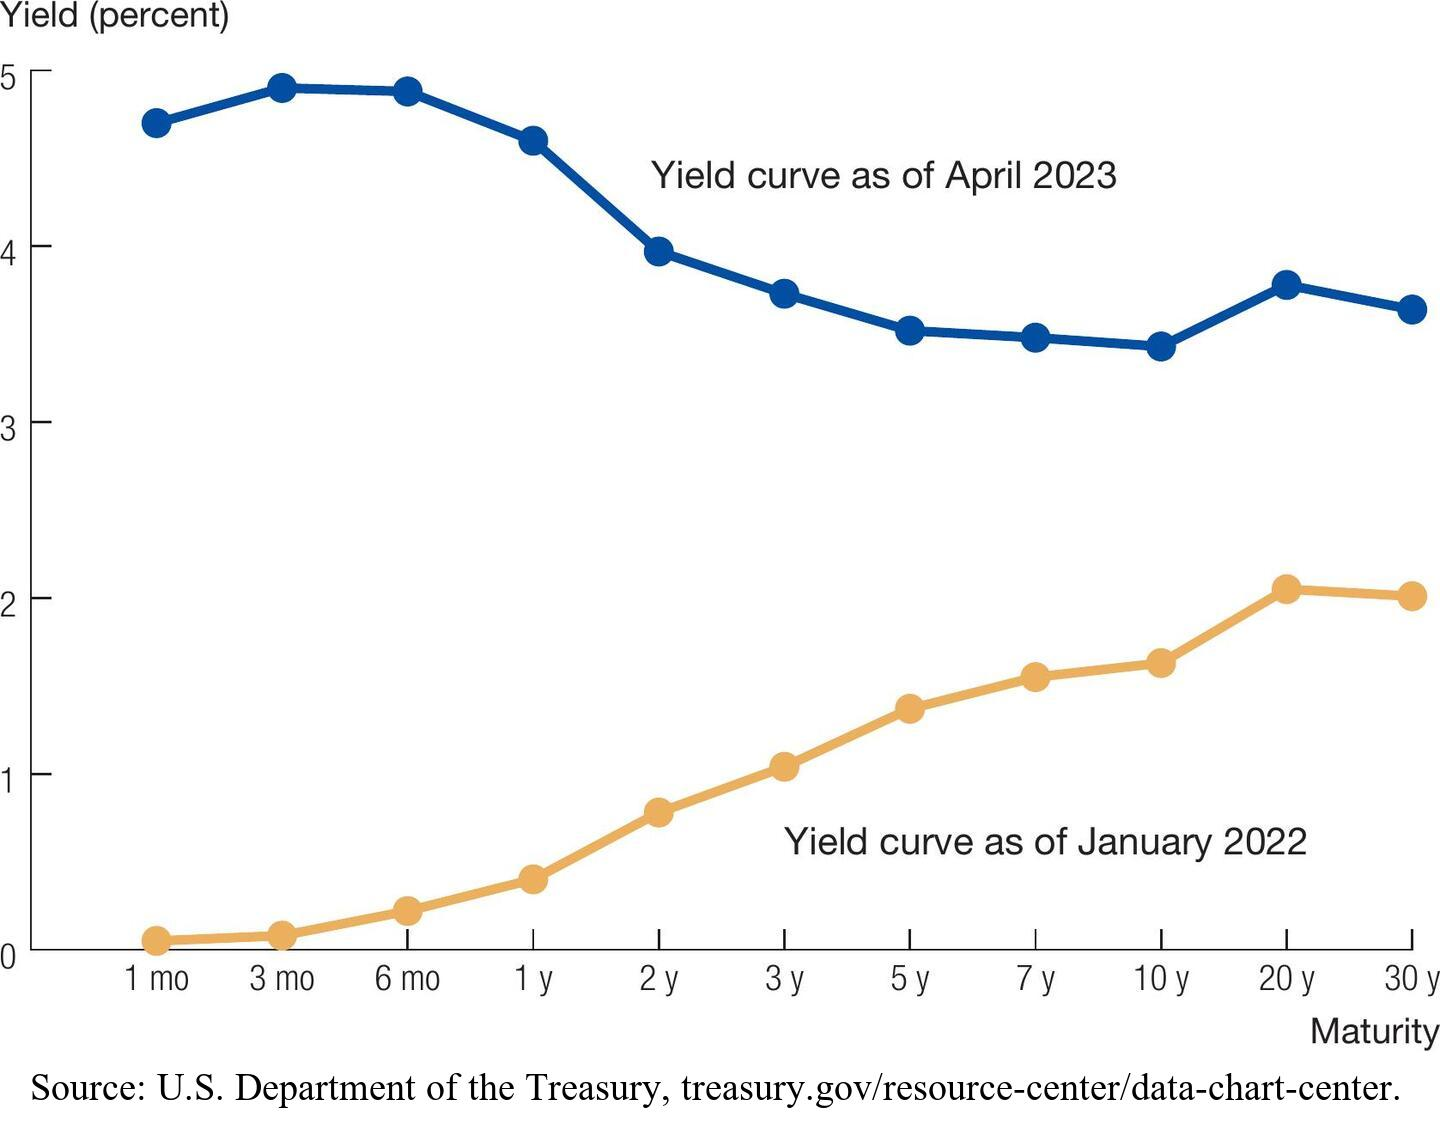
\includegraphics[width=0.7\linewidth]{Figures/MACRO6_FIG12.06}
%	\end{figure}
%\end{frame}

\begin{frame}[wide]{The Phillips Curve}
	\begin{itemize}
		\item The inflation rate is the percent change in the overall price level
		\[\pi_t = \frac{P_{t+1}-P_t}{P_t}\]
		\item Firms set their prices on the basis of
		\begin{itemize}
			\item their expectations of the economy-wide inflation rate ($\pi^e_t$)
			\item the state of demand for their product ($\bar{\nu}\tilde{Y}_t$)
		\end{itemize}
		\item Inflation: $\pi_t = \pi_t^e + \bar{\nu}\tilde{Y}_t$
		\item When the economy is in downturn ($\tilde{Y}<0$), firms would lower their price to keep the sale (i.e., demand curve shift left)
		\item Otherwise, the firm would set the price based on what they expect the overall inflation is going to be
	\end{itemize}
\end{frame}

\begin{frame}[wide]{The Phillips Curve}
	\begin{itemize}
		\item A simple form of the expected inflation can take form of:
		\[\pi^e_t = \pi_{t-1}\]
		\vspace{4mm}
		\item This form is called the Adaptive Expectations:
		\begin{itemize}
			\item Firms expect next year’s inflation rate to be the same as this year’s inflation rate
			\item Firms adjust their forecasts of inflation slowly
			\item Consistent with our sticky inflation assumption
		\end{itemize}
	\end{itemize}
\end{frame}

\begin{frame}[wide]{The Phillips Curve}
	\begin{itemize}
		\item The Phillips curve describes how inflation evolves over time as a function of short-run output
		\vspace{2mm}
		\item Combine the two equations we had from previous slides
		\[\pi_t = \pi_{t-1} +\bar{\nu} \tilde{Y}_t \]
		\vspace{2mm}
		\item If output is below (above) potential, prices rise more slowly (rapidly) than usual
		\[\Delta \pi_t = \pi_t - \pi_{t-1}=  +\bar{\nu}\tilde{Y}_t \]
		\vspace{2mm}
		\item The Phillips curve can be expressed as $\Delta \pi_t = \bar{\nu}\tilde{Y}_t$
		\vspace{1mm}
		\begin{itemize}
			\item $\bar{\nu}$ indicates the sensitive inflation is to demand conditions
		\end{itemize}
		
	\end{itemize}
\end{frame}

\begin{frame}[wide]{The Phillips Curve}
	\begin{figure}
		\centering
		\includegraphics[width=0.5\linewidth]{"Figures/fig 12_08"}
	\end{figure}
	
\end{frame}

\begin{frame}[wide]{Price Shocks and the Phillips Curve}
	\begin{itemize}
		\item To account for temporary increases in the price of inflation, we can add shocks
		\[\pi_t = \pi_{t-1} + \bar{\nu}\widetilde{Y}_t + \bar{o}\]
		or 
		\[\Delta \pi_t = \pi_t - \pi_{t-1}=  \bar{\nu}\widetilde{Y}_t + \bar{o}\]
		\vspace{3mm}
		\item The actual rate of inflation now depends on three things:
		\vspace{1mm}
		\begin{itemize}
			\item The rate of inflation firms expect (past inflation rate)
			\item Demand conditions (adjustment for the state of the economy)
			\item Shocks to inflation	
		\end{itemize}
	\end{itemize}
\end{frame}

\begin{frame}[wide]{Oil Price Shock}
	\begin{itemize}
		\item A rise in oil prices has an immediate and highly visible impact on many prices in the economy. 
		\begin{itemize}
			\item It changes the price of gasoline, an airline ticket and heating a home, etc
			\item The cost of an increase in oil prices has both direct and indirect effects
		\end{itemize}
	\end{itemize}
	\begin{figure}
		\centering
		\includegraphics[width=0.4\linewidth]{"Figures/fig 12_8"}
	\end{figure}
\end{frame}

\begin{frame}[wide]{Cost-Push and Demand-Pull Inflation}
	\begin{itemize}
		\item Cost-push inflation
		\vspace{2mm}
		\begin{itemize}
			\item Price shocks to an input in production 
			\item Tends to push the inflation rate up
		\end{itemize}
		\vspace{4mm}
		\item Demand-pull inflation
		\vspace{2mm}
		\begin{itemize}
			\item Changes in short-run output
			\item Increases in AD pull up the inflation rate
		\end{itemize}
	\end{itemize}
\end{frame}


\begin{frame}[wide]{The Phillips Curve and the Quantity Theory}
	\begin{itemize}
		\item The quantity theory: a decrease in growth rate of real GDP would lead to an increase in inflation]
		\vspace{2mm}
		\begin{itemize}
			\item According to Milton Friedman, inflation is caused by “too much money chasing too few goods.” 
		\end{itemize}
		\vspace{4mm}
		\item The Phillips curve: a decrease in growth rate of real GDP would lead to a decrease in inflation (Not increase)
	\end{itemize}
\end{frame}

\begin{frame}[wide]{The Phillips Curve and the Quantity Theory}
	\begin{itemize}
		\item In the quantity theory, an increase in real GDP reflects an increase in the supply of goods, which lowers prices
		\vspace{2mm}
		\begin{itemize}
			\item This is a long-run model and is supply-driven view
		\end{itemize}
		\vspace{4mm}
		\item In the Phillips curve, an increase in short-run output reflects an increase in the demand for goods
		\vspace{2mm}
		\begin{itemize}
			\item When firms are faced with an increase in demand, they raise their prices
			\item This is part of our short-run model and is a demand-driven view
			%\item In the long run, $\widetilde{Y} = 0$
		\end{itemize}
	\end{itemize}
\end{frame}

\begin{frame}[wide]{Using the Short-Run Model}
	\begin{itemize}
		\item Combine the components of the short-run model to determine output and inflation to illustrate two example
		\vspace{2mm}
		\begin{itemize}
			\item Disinflation: a sustained reduction in inflation to a stable, lower rate
			\vspace{2mm}
			\begin{itemize}
				\item This is seen in how the economy moved from a period of high and uncertain inflation in the 1970s to an extended period of more than two decades of low and stable inflation
			\end{itemize}
			\vspace{2mm}
			\item Causes of the Great Inflation of the 1970s 
			\vspace{2mm}
			\begin{itemize}
				\item This shows how misinterpreting that decade’s productivity slowdown contributed to the rising inflation
			\end{itemize}
		\end{itemize}
	\end{itemize}
\end{frame}

\begin{frame}[wide]{Inflation in the United States}
	\begin{itemize}
		\item In the 70s, the inflation rise rapidly to the highest level since WWII  
	\end{itemize}
	\begin{figure}
		\centering
		\includegraphics[width=0.7\linewidth]{"Figures/MACRO6_FIG12.09.jpg"}
	\end{figure}
\end{frame}

\begin{frame}[wide]{The Volcker Disinflation}
	\begin{itemize}
		\item Paul Volcker was appointed to chair the Federal Reserve Board of Governors in 1979
		\vspace{2mm}
		\item Inflation in 1979 was over 10 percent, partially due to 
		\vspace{2mm}
		\begin{itemize}
			\item loose monetary policy in previous years, and
			\item oil shocks in 1974 and 1979
		\end{itemize}
		\vspace{2mm}
		\item Volker was supposed to bring inflation back under control
	\end{itemize}
\end{frame}

\begin{frame}[wide]{The Volcker Disinflation}
	\begin{itemize}
		\item The long-run theory of inflation tells us the money supply must be reduced
		\vspace{2mm}
		\begin{itemize}
			\item This requires tight money, or an increase in the nominal interest rate
		\end{itemize}
		\vspace{2mm}
		\item However, the classical dichotomy does not hold in the short run
		\vspace{2mm}
		\begin{itemize}
			\item Due to sticky inflation, increasing the nominal interest rate will increase the real interest rate
		\end{itemize}
		\vspace{2mm}
		\item The real interest rate increase induces a recession
		\vspace{2mm}
		\begin{itemize}
			\item The recession causes negative changes in inflation
			\item As demand falls, firms raise their prices slower to sell more
		\end{itemize}
	\end{itemize}
\end{frame}

\begin{frame}[wide]{Tightening Monetary Policy}
	\begin{itemize}
		\item A rise in the real interest rate causes $R>\bar{r}$ due to sticky inflation
		\item Firms and households put their investment plans on hold, which causes output to fall from point A to point B.	The economy enters a recession
		
	\end{itemize}
	\begin{figure}
		\centering
		\includegraphics[width=0.45\linewidth]{"Figures/fig 12_10"}
	\end{figure}
	
\end{frame}

\begin{frame}[wide]{A Recession and Falling Inflation}
	\begin{itemize}
		\item A recession causes the change in the inflation rate to become negative
		\item If the fall in inflation is persistent and form the expectation going forward, the expectation term in PC would fall as well
	\end{itemize}
	\begin{figure}
		\centering
		\includegraphics[width=0.4\linewidth]{"Figures/fig 12_11"}
	\end{figure}
\end{frame}

\begin{frame}[wide]{The Volcker Disinflation}
	\begin{itemize}
		\item Volcker-style policy can keep the real interest rate high and output below potential, until inflation falls to a more appropriate level
		\vspace{2mm}
		\begin{itemize}
			\item At the cost of a slumping economy
			\item High unemployment and lost output
			\item In a lot of developing countries, it may cause civil unrest 
		\end{itemize}
		\vspace{4mm}
		\item Once inflation has declined sufficiently, real interest rate can fall back to MPK, allowing output to rise back to potential
	\end{itemize}
\end{frame}

\begin{frame}[wide]{The Disinflation over Time}
	\begin{figure}
		\centering
		\includegraphics[width=0.8\linewidth]{"Figures/fig 12_12"}
	\end{figure}
\end{frame}

\begin{frame}[wide]{The Great Inflation of the 1970s}
	\begin{itemize}
		\item Inflation in the United States and in many other industrialized countries was relatively low and stable in the 1950s and 1960s
		\vspace{2mm}
		\item Inflation rose in the 1970s for three reasons:
		\vspace{2mm}
		\begin{itemize}
			\item OPEC coordinated oil price increases: Oil shock
			\item U.S. monetary policy was too loose
			\vspace{1mm}
			\begin{itemize}
				\item The belief at this time was that there was a permanent trade-off between inflation and unemployment
				\item Reducing inflation could only be accomplished by a permanent increase in the rate of unemployment (Paul Samuelson and Robert Solow)
				\item However, new theory showed that disinflation required a temporary recession, not a permanent reduction in output (Milton Friedman, Edmund Phelps, Robert Lucas)
			\end{itemize}
		\end{itemize}
	\end{itemize}
\end{frame}

\begin{frame}[wide]{The Great Inflation of the 1970s}
	\begin{itemize}
		\item Inflation rose in the 1970s for three reasons:
		\vspace{4mm}
		\begin{itemize}
			\item The Federal Reserve did not have perfect information
			\vspace{2mm}
			\begin{itemize}
				\item There was a productivity slowdown that started in the early 1970s ($\bar{Y}$ grow slower than before)
				\item However, this was interpreted as a shock to short-run output ($\widetilde{Y}$), pushing it below zero
				\item Policymakers reduced interest rates to stimulate the economy, which led to higher inflation
			\end{itemize}
		\end{itemize} 
	\end{itemize}
\end{frame}

\begin{frame}[wide]{Mistaking a Slowdown in Potential for a Recession}
	\begin{itemize}
		\item The policymaker thought the short-run output was negative and decided to lower the interest rate
		\item Meanwhile, it may boost short-term output. However, in the long run, the economy experienced a period of high inflation
	\end{itemize}
	\begin{figure}
		\centering
		\includegraphics[width=0.45\linewidth]{"Figures/fig 12_13"}
	\end{figure}
	
\end{frame}

\begin{frame}[wide]{The Great Inflation}
	\begin{figure}
		\centering
		\includegraphics[width=0.75\linewidth]{"Figures/fig 12_18"}
	\end{figure}
	
\end{frame}

\begin{frame}[wide]{The Great Inflation}
	\begin{figure}
		\centering
		\includegraphics[width=0.75\linewidth]{"Figures/fig 12_19"}
	\end{figure}
	
\end{frame}

%\begin{frame}[wide]{The 2001 Recession}
%	\begin{itemize}
	%		\item 
	%	\end{itemize}
%	\begin{figure}
	%		\centering
	%		\includegraphics[width=0.5\linewidth]{"Figures/fig 12_14"}
	%	\end{figure}
%	
%\end{frame}

\begin{frame}[wide]{Microfoundations: Understanding Sticky Inflation}
	\begin{itemize}
		\item Sticky inflation is one of the essential building block of the MP curve, which imply changes in the nominal interest rate affect the real interest rate because inflation does not adjust immediately
		\vspace{5mm}
		\item This is also critical for the Phillips curve, the assumption of adaptive expectations assumes that expectations of inflation adjust slowly over time
	\end{itemize}
\end{frame}

\begin{frame}[wide]{Microfoundations: Understanding Sticky Inflation}
	\begin{itemize}
		\item The classical dichotomy states that changes in nominal variables have only nominal effects
		\vspace{2mm}
		\begin{itemize}
			\item The real side of the economy is determined solely by real forces
			\item If the central bank decides to double the money supply, then all prices can double 
			\item If monetary policy affects real variables, the classical dichotomy fails in the short run
			\begin{itemize}
				\item Explaining this failure is one of the crucial requirements of a good short-run model
			\end{itemize}
		\end{itemize}
	\end{itemize}
\end{frame}

\begin{frame}[wide]{The Classical Dichotomy in the Short Run}
	\begin{itemize}
		\item Can the classical dichotomy hold at all points in time?
		\vspace{2mm}
		\begin{itemize}
			\item All prices, including wages and rental prices, must adjust in the same proportion immediately
		\end{itemize}
		\item However, this most likely not happening. Reasons that the classical dichotomy fails in the short run:
		\vspace{2mm}
		\begin{itemize}
			\item Imperfect info
			\vspace{2mm}
			\begin{itemize}
				\item Firms are constantly being hit by a wide range of individual-specific shocks
				\item Monetary policy may not be one of the most important shocks to consider
				\item Subtle monetary policy changes make price coordination difficult
				\item Also, monetary policy changes occur through the interest rate, not through inflation directly, so implementation also depends on other factors
			\end{itemize}
		\end{itemize}
	\end{itemize}
\end{frame}

\begin{frame}[wide]{The Classical Dichotomy in the Short Run}
	\begin{itemize}
		\item Reasons that the classical dichotomy fails in the short run:
		\vspace{2mm}
		\begin{itemize}
			\item Costs of setting prices
			\begin{itemize}
				\item It is too costly and time-consuming to gather information on every detail affecting a firm, and to figure out the correct price every single day
			\end{itemize}
			\item Contracts
			\begin{itemize}
				\item In the short run, contracts set prices and wages in nominal rather than real terms
			\end{itemize}
			\item Bargaining costs
			\begin{itemize}
				\item Negotiating over prices can be risky for job security
				\item In addition, it is costly and difficult and inefficient on a daily basis
			\end{itemize} 
		\end{itemize}
	\end{itemize}
\end{frame}

\begin{frame}[wide]{The Classical Dichotomy in the Short Run}
	\begin{itemize}
		\item Reasons that the classical dichotomy fails in the short run:
		\vspace{2mm}
		\begin{itemize}
			\item Social norms
			\vspace{2mm}
			\begin{itemize}
				%\item Conventions about fairness and how wages are allowed to adjust
				\item Money illusion refers to the fact that people sometimes focus on nominal rather than real magnitudes
				\item People may feel more strongly about nominal wages, regardless of the overall price level in the economy
			\end{itemize}
		\end{itemize}
	\end{itemize}
\end{frame}

\begin{frame}[wide]{Microfoundations: How Central Banks Control Nominal Interest Rates}
	\begin{itemize}
		\item In the short-run model, we assume the central bank “sets” the nominal interest rate
		\vspace{2mm}
		\item The central bank controls the level of the nominal interest rate by supplying the money that is demanded at that rate
		\vspace{2mm}
		\item Develop a simple money demand and supply model to illustrate that 
		\vspace{1mm}
		\begin{itemize}
			\item Start with the case when central bank control the money supply
		\end{itemize}
	\end{itemize}
\end{frame}

\begin{frame}[wide]{Money Supply and Demand}
	\begin{itemize}
		\item The nominal interest rate is the opportunity cost of holding money
		\vspace{4mm}
		\begin{itemize}
			\item The amount you give up by holding the money instead of keeping it in a savings account
			\vspace{2mm}
			\item Assume you have \$100 remaining after covering your current consumption. You have the option to either retain it as cash or deposit it into a savings account
			\vspace{2mm}
			\item If the interest rate is 1\%, the difference is negligible. However, with an interest rate of 20\%, you would aim to hold as little cash as possible
		\end{itemize}
		\item The price in this market is the interest rate
	\end{itemize}
\end{frame}


\begin{frame}[wide]{Money Supply and Demand}
	\begin{itemize}
		\item The demand for money: decreasing function of the nominal interest rate (i.e, downward sloping)
		\item The supply of money determined by the level of money the central bank provides and is	vertical 
		\item The nominal interest rate is pinned down by the equilibrium in the money market, where households are willing to hold just the amount of currency that the central bank supplies
	\end{itemize}
\end{frame}

\begin{frame}[wide]{Money Supply and Demand}
	\begin{itemize}
		\item If the nominal interest rate $i$ is higher than $i^*$, then households would want to hold their wealth in savings accounts rather than currency, so money supply would exceed money demand
		\begin{itemize}
			\item This puts pressure on the nominal interest rate to fall
		\end{itemize}
		\item If $i$ is lower than $i^*$, money demand would exceed money supply, leading $i$ to rise
	\end{itemize}
	\begin{figure}
		\centering
		\includegraphics[width=0.5\linewidth]{"Figures/fig 12_15"}
	\end{figure}
	
\end{frame}

\begin{frame}[wide]{Changing the Interest Rate}
	\begin{itemize}
		\item To increase interest rates:
		\vspace{2mm}
		\begin{itemize}
			\item The central bank reduces the money supply, which creates an excess of demand over supply
			\item A higher interest rate on savings accounts reduces excess demand
			\item The markets adjust to a new equilibrium
		\end{itemize}
	\end{itemize}
\end{frame}

\begin{frame}[wide]{Raising the Nominal Interest Rate}
	\begin{figure}
		\centering
		\includegraphics[width=0.5\linewidth]{"Figures/fig 12_16"}
	\end{figure}
	
\end{frame}

\begin{frame}[wide]{Why $i_t$ instead of $M_t$?}
	\begin{itemize}
		\item Historically, central banks did in fact focus directly on the money supply
		\vspace{2mm}
		\begin{itemize}
			\item Both in the US and much of Europe in the 1970s and early 1980s
		\end{itemize}
		\vspace{2mm}
		\item The interest rate is crucial even when central banks focus on the money supply
		\vspace{2mm}
		\begin{itemize}
			\item After all, that is the variables affecting economic activity
		\end{itemize}
		\vspace{2mm}
		\item The money demand curve is subject to many shocks, which shift the curve
		\vspace{2mm}
		\begin{itemize}
			\item Changes in price and output (higher demand for good require more cash in advance)
			\item Changes in technology (e.g., advent of ATMs, the increasing use of credit and debit cards, and the increased availability of financial products like mutual funds and money market accounts
			\item In the 80s, economist found that it is very hard to pinpoint the demand curve
		\end{itemize}
	\end{itemize}
\end{frame}

\begin{frame}[wide]{Why $i_t$ instead of $M_t$?}
	\begin{itemize}
		\item With a constant money supply, the nominal interest rate would fluctuate, leading to changes in the real interest rate and changes in output if the central bank did not act
		\vspace{2mm}
		\item By targeting the interest rate directly, the central bank automatically adopts a policy that will adjust the money supply to accommodate shocks to money demand
		\vspace{2mm}	
	\end{itemize}
\end{frame}

\begin{frame}[wide]{Why $i_t$ instead of $M_t$?}
	\begin{itemize}
		\item Such a policy prevents the shocks from having a significant effect on output and inflation and helps the central bank stabilize the economy
		\vspace{2mm}
		\item An expansionary (loosening) monetary policy: Increases the money supply or Lowers the nominal interest rate 
		\vspace{2mm}
		\item A contractionary (tightening) monetary policy: Reduces the money supply or Increases the nominal interest rate		
	\end{itemize}
\end{frame}

\begin{frame}[wide]{Why $i_t$ instead of $M_t$?}
	\begin{itemize}
		\item The money supply schedule is effectively horizontal at a targeted interest rate
		\vspace{2mm}
		\begin{itemize}
			\item When the central bank sets an interest rate, it is willing to supply whatever amount of money is demanded at the interest rate
		\end{itemize} 
	\end{itemize}
	\begin{figure}
		\centering
		\includegraphics[width=0.5\linewidth]{"Figures/fig 12_17"}
	\end{figure}	
\end{frame}

%\begin{frame}[wide]{An Increase in the Investment Rate}
%	\begin{columns} 
%			% Column 1
%			\begin{column}{.5\textwidth}
%				\begin{itemize}
%					\item Suppose the investment rate increases permanently for exogenous reasons ($s'>s$)
%					\begin{itemize}
%						\item The investment curve rotates upward ($\bar{s}'\bar{A}  \bar{L}^{1-\alpha} K_t^\alpha > \bar{s}\bar{A}  \bar{L}^{1-\alpha} K_t^\alpha$)
%						\item The depreciation curve remains unchanged ($\delta K_t$)
%						\item The capital stock increases by transition dynamics to reach the new steady state
%						\begin{itemize}
%							\item This happens because investment exceeds depreciation ($sY_t>\delta K_t$)
%						\end{itemize}
%						\item The new steady state is located to the right
%					\end{itemize}
%				\end{itemize}
%			\end{column}
%			% Column 2    
%			\begin{column}{.5\textwidth}			
%				\begin{figure}
%					\centering
%					\includegraphics[width=1\linewidth]{"Figures/An Increase in the Investment Rate"}
%				\end{figure}
%			\end{column}%
%		\end{columns}
%\end{frame}

%\begin{frame}[wide]{Measuring the State of the Economy}
%	\begin{columns} 
%		% Column 1
%		\begin{column}{.5\textwidth}
%			\begin{table}[htbp]
%				\centering
%				\begin{tabular}{lrrrr}
%					& 2005  & 2006  & 2007  & 2008 \\
%					\hline
%					GDP   & 12.6  & 13.4  & 14.0    & 14.3 \\
%					(in trillions of \$) &       &       &       &  \\
%					Growth rate GDP &       & 0.063 & 0.045 & 0.021 \\
%					\hline
%				\end{tabular}%
%				\label{tab:addlabel}%
%			\end{table}%
%		\end{column}
%		% Column 2    
%		\begin{column}{.5\textwidth}			
%			
%			
%		\end{column}%
%	\end{columns}
%\end{frame}

\begin{frame}[wide]{The Covid-19 Recession}
	Covid-19 Recession 
	\vspace{3mm}
	\begin{itemize}
		\item GDP sharply declined by 10 percent in 2020
		\item  By 2022, GDP had returned to trend
		\item  Inflation declined somewhat in 2020 at the beginning of the recession
		\item  By 2021, inflation started rising and continued to levels not seen since the 1970s
	\end{itemize}
	\vspace{4mm}
	Why did GDP fall sharply and then quickly rebound?
	\vspace{3mm}
	Why did inflation initially decline in 2020, and then rise quickly in 2021 and 2022?
\end{frame}

\begin{frame}[wide]{Covid-19 Recession and Real GDP in the United States}
	\begin{figure}
		\centering
		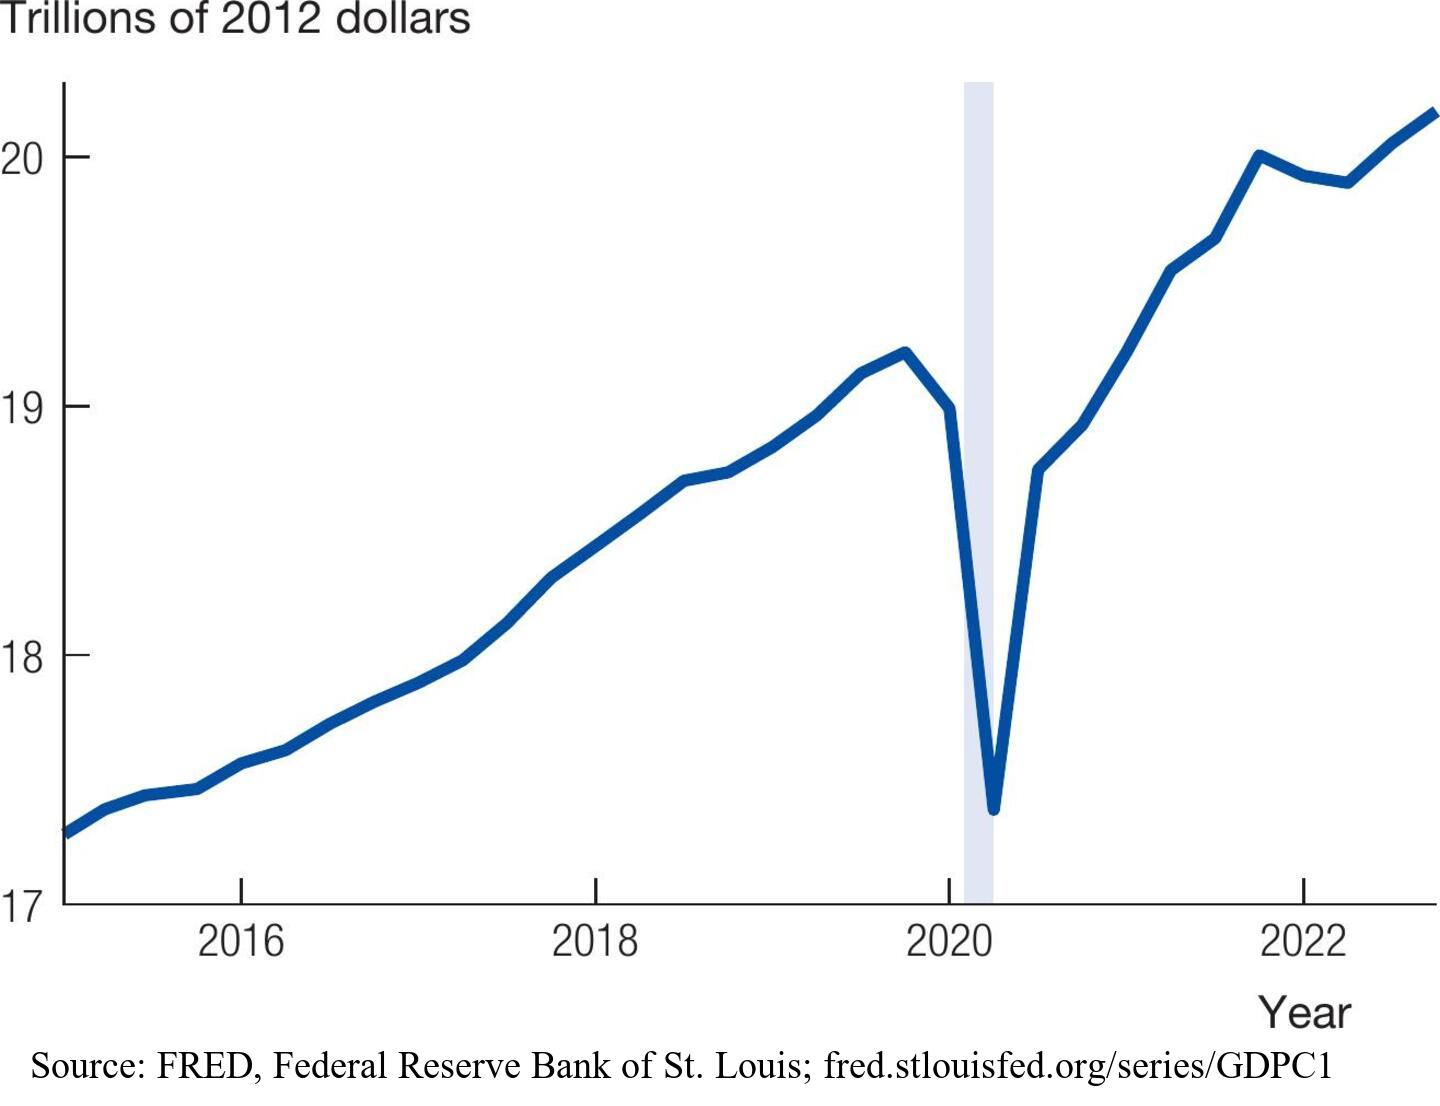
\includegraphics[width=0.7\linewidth]{Figures/MACRO6_FIG12.14}
	\end{figure}
\end{frame}

\begin{frame}[wide]{Covid-19 Recession and Consumer Price Index Inflation in the U.S.}
	\begin{figure}
		\centering
		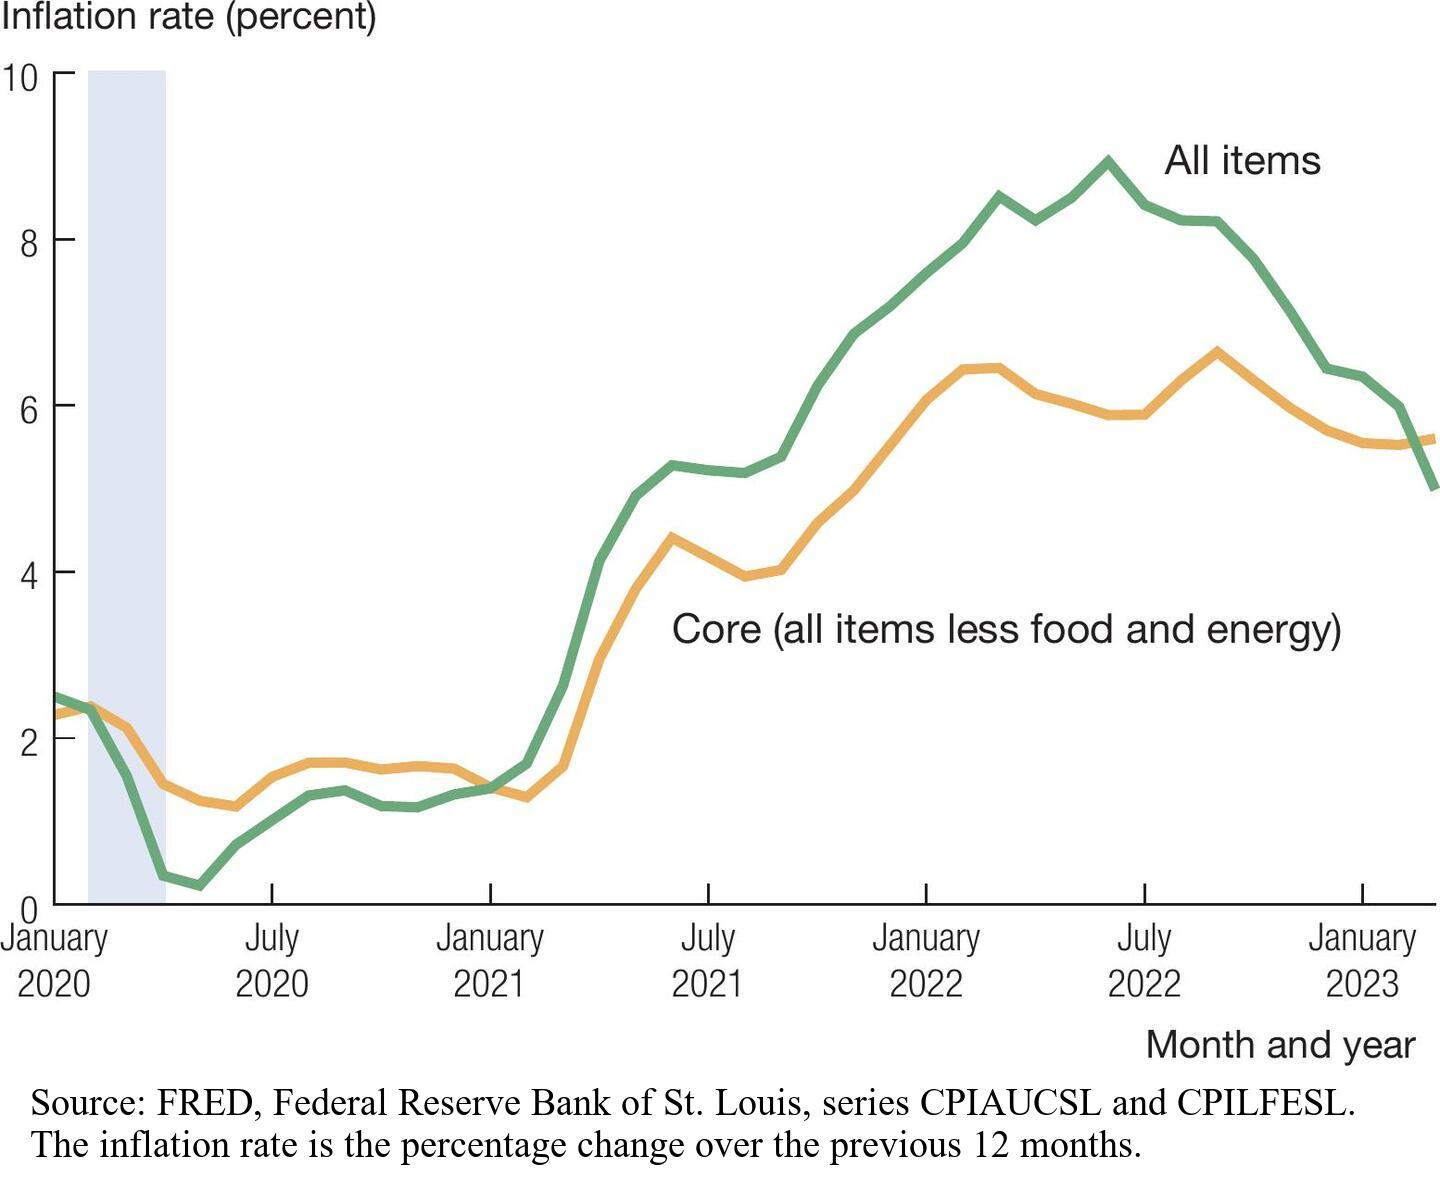
\includegraphics[width=0.7\linewidth]{Figures/MACRO6_FIG12.15}
	\end{figure}
\end{frame}

\begin{frame}[wide]{Covid-19 as an Aggregate Demand Shock}
	Covid-19 acted as a ``tax" on consumption
	
	\vspace{5mm}
	\begin{itemize}
		\item Possibility of contracting Covid-19 reduced in-person retail, in-person dining, travel, and in-person entertainment activity
		\vspace{2mm}
		\item Consumption fell sharply
		\vspace{4mm}
		\[\bar{a}_C \downarrow \to \bar{a} \downarrow = \tilde{Y}_t \downarrow \to \pi_t \downarrow\]
	\end{itemize}
\end{frame}

\begin{frame}[wide]{Covid-19 as a Shock to $\bar{Y}$}
	Covid-19 acted as a ``tax" on working
	\vspace{5mm}
	\begin{itemize}
		\item Possibility of contracting Covid-19 if you left home to go to work reduced employment both voluntarily and involuntarily
		\vspace{2mm}
		\item Employment declined sharply, reducing production
		\vspace{2mm}
		\item $\bar{Y}$ declines
	\end{itemize}
\end{frame}

\begin{frame}[wide]{U.S Federal Government Spending as a Share of GDP}
	\begin{itemize}
		\item The sharp increase in government spending during the Covid-19 pandemic buffered the economy from negative economic impacts
		\item Although unemployment reached levels not seen since the Great Depression, household incomes increased for many because of government intervention
		\begin{figure}
			\centering
			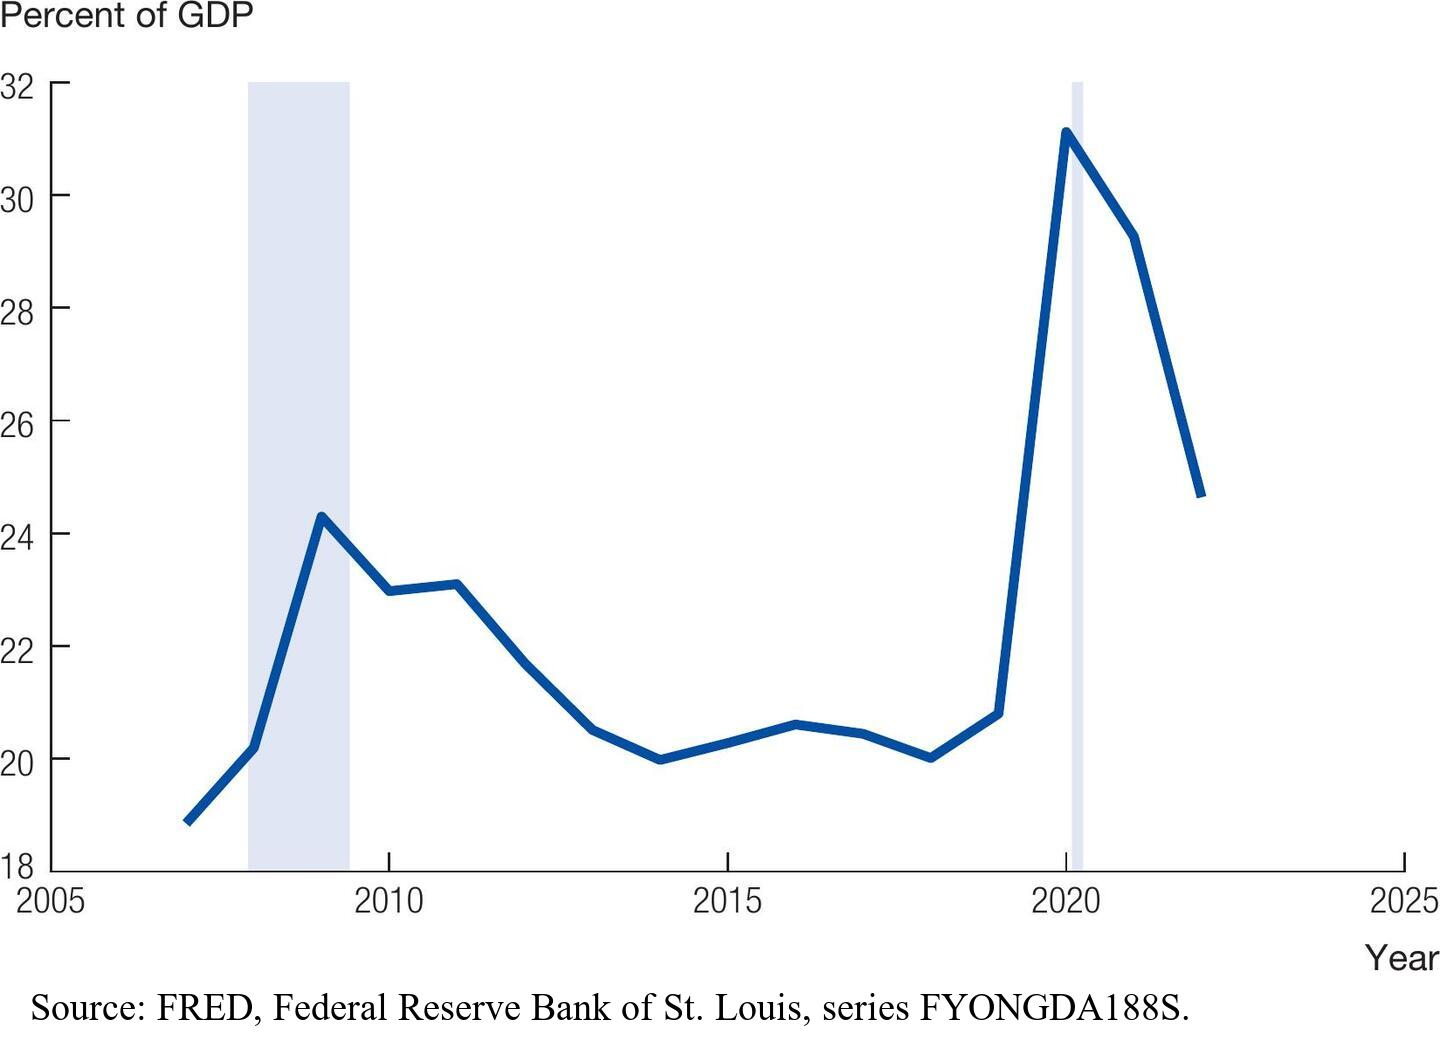
\includegraphics[width=0.5\linewidth]{Figures/MACRO6_FIG12.16}
		\end{figure}
		\item Resulting an increase in $\bar{a}_g$
	\end{itemize}
\end{frame}

\begin{frame}[wide]{Government's Responses }
	Another reason for the strong economic recovery was government policy
	\vspace{4mm}
	\begin{itemize}
		\item Government spending as share of GDP increased from 22 percent in 2019 to 32 percent in 2020
		\vspace{2mm}
		\item Loans, unemployment benefits, and direct transfers to businesses and individuals allowed for continued consumption
		\vspace{2mm}
		\item Disposable personal income increased from 2020 to 2021 despite a 15 percent unemployment rate
	\end{itemize}
\end{frame}

\begin{frame}[wide]{Income and Consumption}
	\begin{itemize}
		\item The three spikes in disposable personal income correspond to three separate direct payments from government to households
		\item The simultaneous increase in disposable personal income and decrease in consumption resulted in increased household savings and a decline in poverty
	\end{itemize}
	\begin{figure}
		\centering
		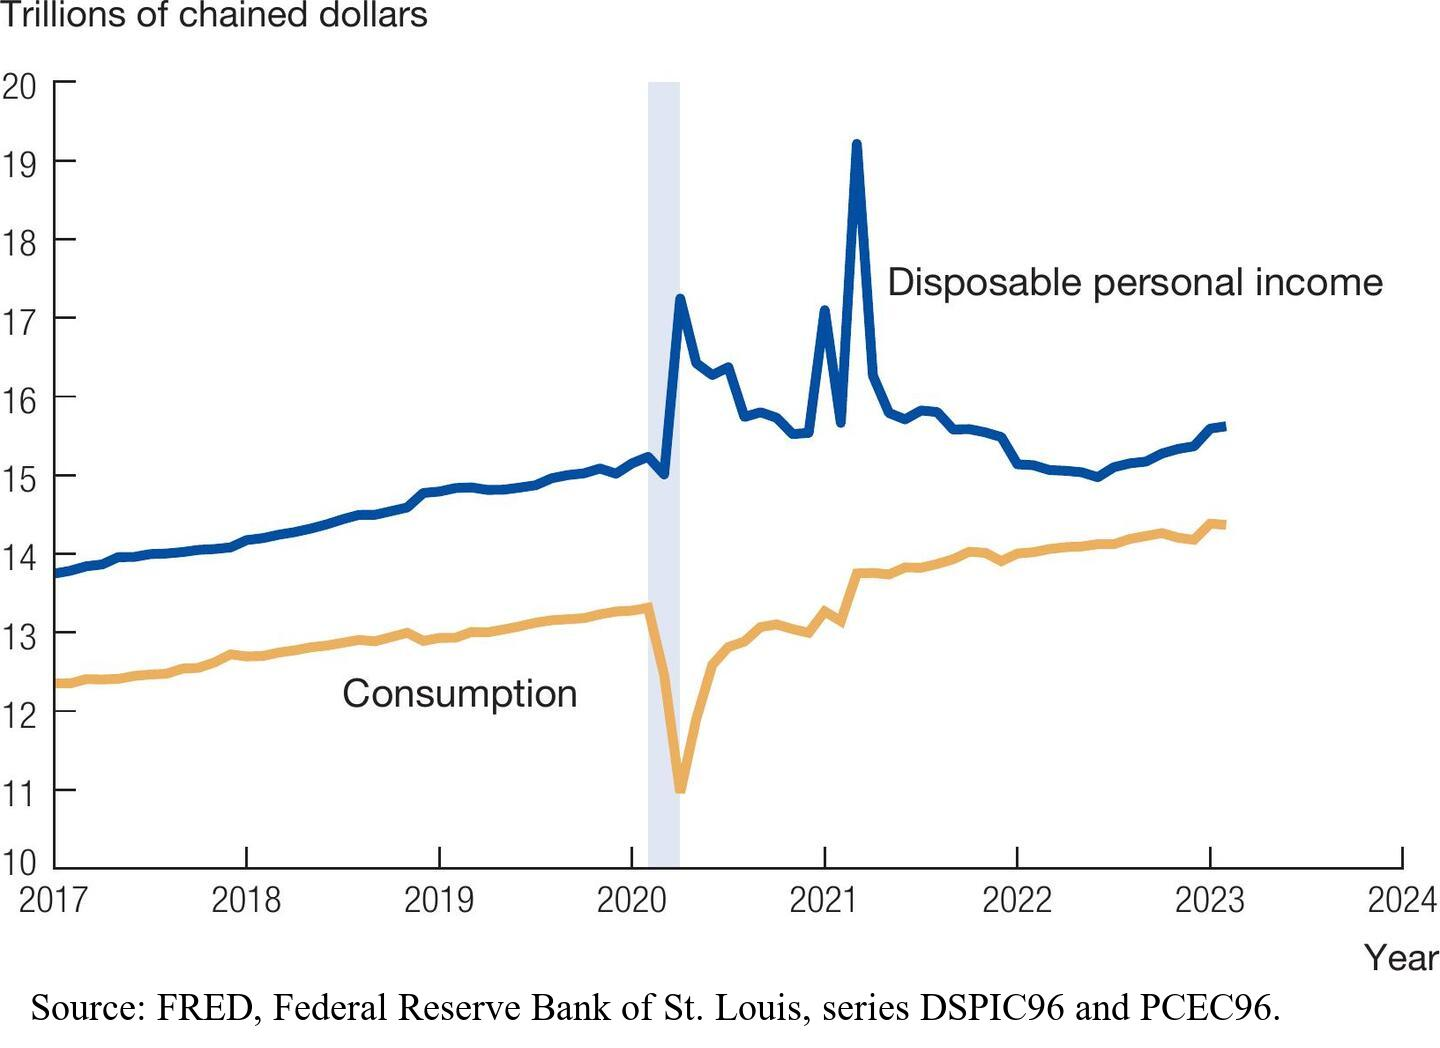
\includegraphics[width=0.5\linewidth]{Figures/MACRO6_FIG12.17}
	\end{figure}
\end{frame}

\begin{frame}[wide]{Central Bank's Responses  }
	\begin{itemize}
		\item Bank of Canada lowered the bank rate from 2\% to close to 0\%
		\vspace{4mm}
		\begin{figure}
			\centering
			% [Figure not available] \includegraphics[width=1\linewidth]{Figures/Bank_Rate_Covid}
		\end{figure}
		\item The MP curve shift down
	\end{itemize}
\end{frame}

\begin{frame}[wide]{Combined Shock}
	\begin{itemize}
		\item The economy was shocked with
		\begin{itemize}
			\item a decrease in $\bar{a}_c$
			\item a decrease in $\bar{Y}$
		\end{itemize}
		\item The government and central bank responses with:
		\begin{itemize}
			\item an increase in $\bar{a}_g$
			\item a decrease in $R_t$
		\end{itemize}
		\item In combination, the economy experienced
		\begin{itemize}
			\item A large fall in current output $Y_t$
			\item Mild decrease in $\tilde{Y}_t$ as the decrease in $\bar{Y}$ and government/central bank helps lowered the impact
			\item Resulting a mild decrease in $\Delta \pi_t$
		\end{itemize}
	\end{itemize}
\end{frame}

\begin{frame}[wide]{The Rapid Recovery of GDP }
	\begin{itemize}
		\item Production can recover quickly from negative shocks
		\vspace{2mm}
		\begin{itemize}
			\item Happens after every weekend
			\item In Europe, many manufacturers shut down in August for vacation and restart in September
		\end{itemize}
		\vspace{4mm}
		\item The Covid-19 recession was short-lived because people quickly returned to normal economic activity
		\vspace{2mm}
		\begin{itemize}
			\item Improved scientific understanding of the virus
			\item Widespread availability of masks
			\item Effective vaccines
		\end{itemize}		
	\end{itemize}
\end{frame}


\begin{frame}[wide]{The Return of Inflation}
	\begin{itemize}
		\item After decades of 2 percent inflation, the increase in inflation rates in 2021–2022 surprised most observers
		\vspace{6mm}
		\item How did this happen?
		\vspace{2mm}
		\begin{itemize}
			\item Covid-19 pandemic interfered with global supply chains
			\item Energy price shocks associated with the war in Ukraine
			\item Demand for goods outpaced production
		\end{itemize}
	\end{itemize}
\end{frame}

\begin{frame}[wide]{Next Lecture}
	\begin{itemize}
		\item Next lecture will cover Ch.13
	\end{itemize}
\end{frame}

\end{document}